\documentclass{pset}

\usepackage{preamble}
\usepackage[new]{old-arrows}
\graphicspath{ {../}}
\renewcommand{\hmwkTitle}{2nd\ hw}
\renewcommand{\hmwkDueDate}{February 12, 2014}
\renewcommand{\hmwkClass}{Algebraic Topology}
\renewcommand{\hmwkClassTime}{Section 1.1}
\renewcommand{\hmwkAuthorName}{DarQ}



\begin{document}

\maketitle

\pagebreak 

\begin{problem}
    \begin{enumerate}
        \item The statement is only true for $n \geq 3$
        \item With the above modification, we know the statement is true if only one point is removed. We also know the spaces are path connected hence our choice of basepoint is immaterial, and it suffices to prove that they have trivial fundamental group.
        
        Now suppose the statement is true still if $k$ points are removed. And let $X$ be $\bR^n$ with $k+1$ points removed. Let's split $\bR^n$ into two overlapping sets:
        \[A = (-\i, 1)\times\bR^{n-1}\]
        and
        \[B = (-1, \i)\times\bR^{n-1}\]
        which are both homeo $\bR^n$ and make sure one of the removed points is in the complement of $A$ and the rest is in the complement of $B$. Thereby, we get 2 path-connected open sets $A'$ and $B'$ whose intersection is path connected such that $A'$ is homeo $\bR^n$ with $k$ points removed and $B'$ is homeo $\bR^n$ with one point removed. Hence, if you take any loop based at, say, $0$, due to lemma 1.15 (see hatcher) would be homotopic to a product of loops each of which is entirely contained in either $A'$ or $B'$ but any such loop is homotopic to the constant loop and hence we are done.
    \end{enumerate}
\end{problem}

\begin{problem}
    \begin{enumerate}
        \item Let $T$ be the linear transformation associated with $A$. First, we notice that $T$ takes vectors with non-negative entries to vectors with non-negative entries. Therefore, if we let
        \[Q^1 = \{(x, y, z)\in\bR^3|x,y,z\geq 0\}\]
        then
        \[T(Q^1) \subset Q^1\]
        let $\rho\colon \bR^3\setminus \{0\}\longrightarrow S^2$ be the continuous map defined as
        \[\rho(\vec{x}) = \frac{\vec{x}}{\norm{\vec{x}}}\]
        let's now restrict $T$ to $Q^1 \cap S^2$ which is homeo $D^2$. We then get a continuous map
        \[Q^1 \cap S^2 \xlongrightarrow{T} Q^1 \setminus \{0\} \xlongrightarrow{\rho} Q^1 \cap S^2\]
        hence, due to Brouwer's fixed point theorem, there exists a unit vector such that
        \[T(\vec{x}) = a\vec{x}\]
        for some $a\in\bR$
        
        \item It suffices to prove that the previous map:
        \[Q^1 \cap S^2 \xlongrightarrow{T} Q^1 \setminus \{0\} \xlongrightarrow{\rho} Q^1 \cap S^2\]
        is well-defined still. And indeed it is since invertible matrices don't send non-zero vectors to zero.
    \end{enumerate}
\end{problem}
\begin{problem}
    We're first going to do b and c and then from that we're going to derive a.
    \begin{enumerate}
        \setcounter{enumi}{1}
        \item Define the deformation retraction $f_t:I^2 \to I^2$ of the unit square onto its midline as:
        \[f_t(x, y) = 
        \begin{cases}
            \big(0.5 - (1-t)(0.5-x), y\big) & x \leq 0.5 \\
            \big(0.5 + (1-t)(x-0.5), y\big) & x \geq 0.5 
        \end{cases}
        \]
        and then compose that with an appropriate quotient map to go to a Möbius strip.

        \item This follows immediately from b. and Proposition 1.18.
        \setcounter{enumi}{0}
        \item Let $\omega$ and $\varsigma$ be representative loops of the generators of $\pi_1(M)$ and $\pi_1(\partial M)$ respectively. Notice that, through $f_t$ defined previously, $\varsigma \simeq 2\omega$. Now supposing such a retraction $r\colon M\to\partial M$ exists: $r\omega$ must be a loop in $\partial M$ and since $2\omega \simeq \varsigma$ 
        \[2r\omega\simeq r\varsigma = \varsigma\]
        but since $2x=1$ doesn't have a solution in $\bZ$ we arrive at a contradiction.
    \end{enumerate}
\end{problem}

\begin{problem}
    \begin{enumerate}[label=1.1.\arabic*]
        \item This is essentially the exact same proof as the proof that traversing a loop and then traversing it backwards is homotopic to the constant loop except for paths general and not just loops.
        \item Suppose $h_0\simeq h_1$ through the homotopy $h_t$ then $h_0\cdot f\cdot\bar{h}_0\simeq h_1 \cdot f \cdot \bar{h}_1$ through $h_t \cdot f \cdot \bar{h}_t$
        \item Let $e$ be a representative loop of the identity in $\pi_1(X)$ and $f$ be any representative loop. Since $f$ has the same endpoint as the constant loop we get that $\beta_f = \beta_e$ hence for any loop $g$
        \[[f \cdot g \cdot \bar{f}] = \beta_f(g) = \beta_e(g) = [e \cdot g \cdot \bar{e}] = [g]\]
        And therefore, the $\pi_1(X)$ is Abelian.
        \setcounter{enumi}{5}
        \item Maps $S^1 \to X$ could just be identified with paths $I \xlongrightarrow{f} X$ such that $f(0) = f(1)$ (i.e. loops), so we're going to work with that. First, we note that any path is homotopic to a map constant at its starting point or ending point, i.e.
        \[x \mapsto f(0) \simeq f \simeq x \mapsto f(1)\]
        through the homotopy
        \[f_t(x) =
        \begin{cases}
            f(x) & t<x \\
            f(1-t) & x \leq t \leq 1
        \end{cases}
        \]
        or 
        \[f_t(x) =
        \begin{cases}
            f(t) & t<x \\
            f(x) & x \leq t \leq 1
        \end{cases}
        \]
        So if you let $f$ be any loop in $X$ and $h$ be a path from $f(0)$ to $x_0$ then
        \[[f] = [h \cdot f \cdot \bar{h}] \in \pi_1(X, x_0)\] 
        \setcounter{enumi}{15}
        \item 
        \begin{enumerate}
            \item if $\bR^3$ deformation-retracts to $A$ then that would mean they have the same fundamental group but any loop in $\bR^3$ is nullhomotopic, as in $\pi_1(\bR^3) = 0$ whereas $\pi_1(A) \cong \bZ$ since it's homeo $S^1$
            \item $D^2$ is contractible hence
            \[\pi_1(S^1 \times D^2) \cong \pi_1(S^1) \cong \bZ\]
            whereas
            \[\pi_1(S^1 \times S^1) \cong \bZ^2\]
            hence the two spaces aren't even homotopy equivalent
            \item Any loop in $A$ is nullhomotopic in $S^1 \times D^2$ hence the inclusion $A \hookrightarrow X$ induces a trivial homomorphism but since $\pi_1(S^1 \times D^2) = \bZ = \pi_1(A)$ the induced homomorphism wouldn't be injective which is what would've happened if there existed a retraction from $X$ to $A$
            \item $D^2 \vee D^2$ is contractible hence
            \[\pi_1(D^2 \vee D^2) = 0\]
            whereas $\pi_1(S^1 \vee S^1)$ contains at least $\bZ$ as a subgroup generated by the loop going through one of the circles once.
            \item $X$ here is deformation-retracts onto $S^1$ (see figure) hence
            \[\pi_1(X) = \bZ\]
            whereas 
            \[\pi_1(S^1 \vee S^1) \cong <a, b>\]
            
            \centering
            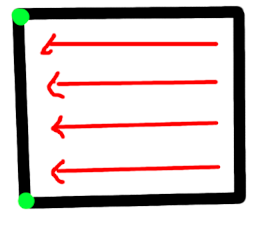
\includegraphics[width=6 cm]{deformation.png}

            we identify the two green dots and the red arrows define a deformation-retraction of the square to a line.
        \end{enumerate}
        \setcounter{enumi}{17}
        \item We're going to split $X$ into two path-connected open subsets with a path connected subsets, one is homeomorphic to $\operatorname{Int} D^n$ and the other deformation retracts to $A$. To do this, consider the characteristic map $\Phi$ defined as the composition of maps:
        \[D^n \longhookrightarrow A \amalg D^n \longrightarrow A \cup_\varphi D^n\]
        where $\varphi\colon \partial D^n \to A$ is the attachment map. Let $\mathbf{A}$ be the image of $(1-\epsilon, 1] \times \partial D^n$ (according to the "spherical" coordinates) under $\Phi$; $\mathbf{A}$ is open since its preimage under the quotient map, $A \cup (1-\epsilon, 1] \times \partial D^n$, is open. Now let $\mathbf{B}$ be the image of $\operatorname{Int} D^n$ under $\Phi$. Now we get
        \[X = \mathbf{A} \cup \mathbf{B}\]
        and $\mathbf{A}$, $\mathbf{B}$, and $\mathbf{A \cap B}$ are all path-connected. The last one is due to the fact that
        \[\mathbf{A \cap B} = \Phi\big((1-\epsilon, 1] \times \partial D^n \cap \Int D^n \big) = \Phi\big((1-\epsilon, 1) \times \partial D^n \big)\]
        and the fact that the image of path-connected sets are path-connected. Moreover, $\mathbf{A}$ deformation-retracts to $A$: take the deformation-retraction $f_t\colon (1-\epsilon, 1] \times \partial D^n \to \mathbf{A}$ 
        \[f_t(r, \theta) = \Phi\big(t+r(1-t), \theta\big)\]
        defined on the "spherical" coordinates where $r\in (1-\epsilon, 1]$ and $\theta\in\partial D^n$ and since $f_t$ is constant on the fibers of $\Phi$, through the characteristic property of quotient spaces there exists a unique deformation-retraction
        \[\tilde{f}_t\colon \mathbf{A \longrightarrow A}\]
        from $\mathbf{A}$ onto $A$.
        
        Now to prove the theorem you merely need to choose a base point in $\mathbf{A \cap B}$ (it doesn't matter where we choose our basepoint since $X$ is path connected) and due to lemma 1.15 any loop in $X$ can be broken down to a loop entirely contained in either $\mathbf{A}$ or $\mathbf{B}$ and since $\mathbf{B}$ is contractible any loop in $X$ is homotopic to a loop in $\mathbf{A}$ and is therefore homotopic to a loop in $A$, and we are done.

        Now onto applications:
        \begin{enumerate}
            \item $\pi_1(S^2 \vee S^1)$ is going to at least have $\bZ$ as a subgroup generated by looping around $S^1$ once and since $S^2 \vee S^1$ can be obtained by attaching a 2-cell to a single point of $S^1$ and since $S^1$ is path connected then the inclusion $S^1 \to S^2 \vee S^1$ induces a surjection
            \[\bZ \cong \pi_1(S^1) \twoheadrightarrow \pi_1(S^2 \vee S^1)\]
            and since the latter has a trivial kernel that surjection is an isomorphism.
            \item 
        \end{enumerate}
    \end{enumerate}
\end{problem}
\begin{problem}
    \begin{enumerate}
        \item This part is just a bunch of calculations, so I'll just lay them out here in succession
        \begin{enumerate}[label=\roman*.]
            \item showing \(1_\times = 1_\circ\):
            \begin{align*}
                (1_\circ \circ 1_\times) \times (1_\times \circ 1_\circ) &= (1_\circ \times 1_\times) \circ (1_\times \times 1_\circ) \\
                (1_\circ \circ 1_\times) \times (1_\times \circ 1_\circ) &= 1_\times \\
                (1_\circ \times 1_\times) \circ (1_\times \times 1_\circ) &= 1_\circ 
            \end{align*}

            \item Showing the operations coincide:
            \begin{align*}
                a \times b &= (a \circ 1_\circ) \times (1_\circ \circ b) \\
                &= (a \times 1_\circ) \circ (1_\circ \times b) \\
                &= (a \times 1_\times) \circ (1_\times \times b) \\
                &= a \circ b
            \end{align*}
            and to see that the operations are commutative:
            \begin{align*}
                a \times b &= (1_\circ \circ a) \times (b \circ 1_\circ) \\
                &= (1_\circ \times b) \circ (a \times 1_\circ) \\
                &= b \circ a \\
                &= b \times a
            \end{align*}
            \item showing the operations are associative:
            \begin{align*}
                a \times (b \times c) &= (a \circ 1_\circ) \times (b \circ c) \\
                &= (a \times b) \circ (1_\circ \times c) \\
                &= (a \times b) \times c 
            \end{align*}
        \end{enumerate}
        \item
        \begin{enumerate}[label=\roman*.]
            \item we just need to verify the axioms of group:
            \begin{itemize}
                \item $\Omega(G, x_0)$ is closed under $\times$ since group multiplication is continuous.
                \item The identity is the constant loop $\iota(t)=x_0$ since for all loops $f\in\Omega(G, x_0)$
                \[(f\times\iota)(t) = f(t)\iota(t) = f(t)x_0 = f(t)\]
                \[(\iota\times f)(t) = \iota(t)f(t) = x_0f(t) = f(t)\]
                \item the inverse of a loop $f$ is the loop $\bar{f}(t) = f(t)^{-1}$. This is valid since the map that takes an element to its inverse is continuous.
                \item Associativity follows from the associativity of $G$.
            \end{itemize}
            \item $\pi_1(G, x_0)$ is just $\Omega(G, x_0)$ but quotiented by the homotopy relation, so we need only verify that $[f] \times [g] = [f \times g]$ is well-defined. Thereby, suppose $f_0 \simeq f_1$ by a homotopy $f_t$ and same for $g_0 \simeq g_1$. Hence,
            \[f_0 \times g_0 \simeq f_1 \times g_0\]
            through the homotopy $f_t \times g_0$, and
            \[f_1 \times g_0 \simeq f_1 \times g_1\]
            through the homootpy $f_1 \times g_t$. Therefore,
            \[f_0 \times g_0 \simeq f_1 \times g_1\]
            and we are done.
            \item one need only notice that, for $f, g, h, k \in \pi_1(G, x_0)$,
            \[\bigl((f \circ g) \times (h \circ k)\bigr)(t) = 
            \begin{cases}
                f(2t)h(2t) &t\in[0, 1/2] \\
                g(2t-1)k(2t-1) &t\in[1/2, 1]
            \end{cases}
            \]
            and that
            \[\bigl((f \times h) \circ (g \times k)\bigr)(t) = 
            \begin{cases}
                f(2t)h(2t) &t\in[0, 1/2] \\
                g(2t-1)k(2t-1) &t\in[1/2, 1]
            \end{cases}
            \]
            meaning they're the exact same function.
            \item This follows immediately from a.ii.
        \end{enumerate}
        \item This one follows the same logic as the last, so I thought it superfluous to type it again :).
    \end{enumerate}
\end{problem}

\begin{align*}
    X_n' &= X_n' \cup \bigcup_{e\in \mathcal{E}'} e, & X_n' &= X_n' \cup \bigcup_{e\in \mathcal{E}'} e.
\end{align*}
\end{document}
